% \section{Market Survey}
% Market Survey goes here, I think it should be called Market VISIBILITY study.

% In this chapter, you survey the related market to your project. Other similar tools/platforms should be discussed. The drawbacks within them, which justify the need of you project, should be given.

% In this space, before the first section, write an introductory paragraph on the project market
Hiring applications and platforms’s market has been growing since 2012, The leading companies or platforms are “ideal”\cite{ideal}, “SparkHire”\cite{SparkHire}, “SmartRecruiters”\cite{SmartRecruiters} and “Outmatch”. Each of them provides one or more services(s) to help in the hiring process. These services could be:

\begin{itemize}
  \item CV ranking: rank CVs using artificial intelligence and some common based rules.
  \item Video analysis: analyze the video and recognizing emotions expressed on it.
  \item A one-way video interview: based on questions, the interviewee records a video and answers those questions, and the system analyzes the responses.
  \item Live video interview: the video may be recorded to refer to later.
  \item Question/Answering System: it provides Q\&A in a written format and analyzes answers to predict personalities.
  \item Interview Collaboration: consult and get advised by discussing with other interviewers.
  \item Chat bot: an expert system built using artificial intelligence, used to simulate digital conversations and interactions with applicants.
\end{itemize}

“iHire”, provides CV ranking, video analysis, and Question/Answering system.



\section{Targeted Customers}
% In this section, mention who are the intended customers of your project and explain how these customers benefit from it

Our targeted customers are companies. Our initial market will be the Egyptian market. The Egyptian market is a small niche with low competition. We provide service to these companies for a monthly/yearly subscription or by a contract. They can use our website or simply use our API. 

\section{Market Survey}
% In this section, list the competitive products to your work. Similar commercial tools/platforms should be mentioned and discussed. Write a subsection for everyone of them and explain its pros and cons in that subsection

\subsection{ideal}
"ideal" provides an AI solution to rank resumes given the job description. Ranking improves as the system goes and as it learns from the previous recruiting data and comparing with final employing decisions. It has : \textbf{CV ranking} and \textbf{Chat bot}.\newline

It does not provide these services: \textbf{Video analysis} and \textbf{Question/Answering System}.
They have different pricing depending on their customers and their project.

\subsection{SparkHire}
This system provides a tool to create video interviews and facilitates reviewing them easier. It has: \textbf{A one-way video interview},  \textbf{Live video interview} and \textbf{Interview Collaboration}.\newline

It does not provide these services:
\textbf{CV ranking}, \textbf{Question/Answering System} and \textbf{Chat bot}.
Their pricing is €249/month.\cite{SparkHire Pricing}

\subsection{SmartRecruiters}
"SamrtRecruters" is an applicant tracking systems (ATS) that provides a convenient way to handle data of a large volume of applicants. Some of them provide ways of filtering the applicants based on keywords in their resumes. It has: \textbf{CV ranking} and \textbf{Chat bot}. \newline

It doesn't provide these services:
\textbf{Video analysis} and \textbf{Question/Answering System}.
Their pricing depends on their customers and their projects but on average \$10,000/year.\cite{SmartRecruiters Pricing}

\subsection{Outmatch}
This system provides tools that assess the applicants’   personalities and technical skills. It has:
\textbf{Question/Answering system} and \textbf{Live Video interview}. \newline

It does not provide these services:
\textbf{CV ranking} and \textbf{Video analysis}.
They have different pricing depending on their customers and their project.

\section{Business Case and Financial Analysis}

% In this section you describe the success of establishing a company to sell your product (or service) 

% Two Aspects must be addressed
% Business Case:   Based on Market survey above you should anticipate how many products you will sell over the next 5 years and how will you set your price to counter the competition.

% Financial Analysis: Based on the business case we must anticipate 
% The Capex (Capital Expenditure):  These are one-time spending that you pay for development and buying things for the company
% The Opex (Operational Expenses): These are recurring payments for salaries and marketing and … etc.
% Then you create what we call a cash flow table (on an excel sheet). In this sheet you put down your monthly capex and opex on a set of rows and your reveneus (money you get back from selling product/services) on another set of rows.
% The difference between both sums is your profit before tax.
% It is likely that this difference is negative at beginning until your sales increase and counter the expenses.
% From this cash flow analysis you find the date of the break even point which is the date at which all the money you get back equals the money you spent. From that date onward you will be making true profit.

\subsection{Business Case}
After reviewing our competitors pricing and product, we set our price €208 $\simeq$ 3848L.E. /month. According to CEIC, there are about 521 companies in Egypt in all fields ( construction \& material, goods, automobile ,technology,...), According to the feasibility study in Appendix E, 15\% of them will buy our services which gives a total revenue of 300144 L.E./month.

\subsection{Financial Analysis}

We will buy 4 laptops, each costing 10,000 L.E., and will renew these laptops after 3 years, which means we will pay 1112 L.E. monthly. Concerning salary we will start with our team which consists of 4 members each with a salary 8000 L.E. monthly. And concerning bills will be on average 1000 L.E., the marketing and sales will be 6000L.E/month and 8000 L.E/month respectively, concerning server hosting, we will hire 5 servers with Specs (CPU 2 vCPU, RAM 4GB, Disk 100GB, OS Linux, Network speed 200 Mbps) with price €22/month\cite{Server pricing} this costs around 2040 L.E. \newline

Below we show a figure of the cash flow for 13 months.

\begin{figure}[h!]
\centering
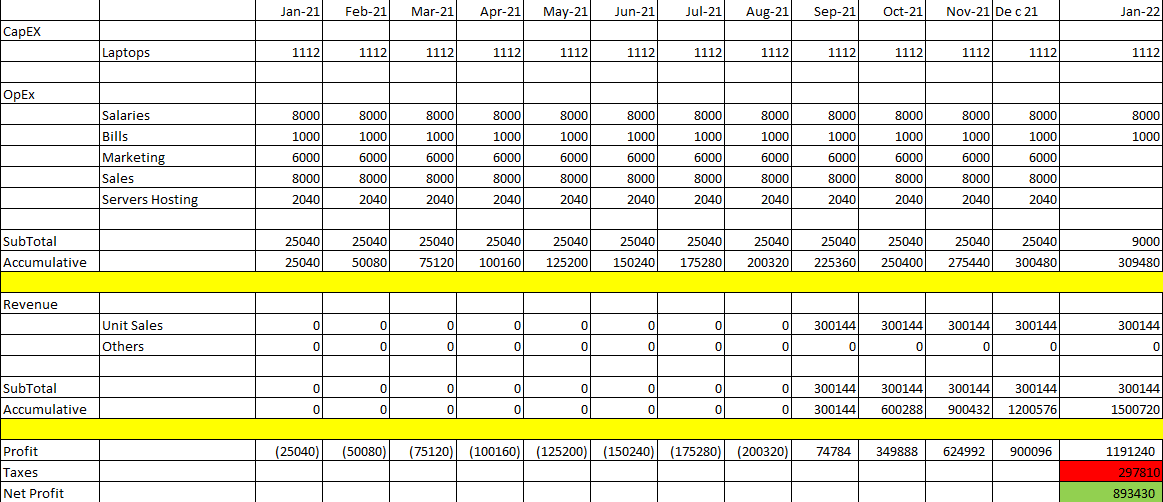
\includegraphics[width=1.1\textwidth]{images/Cash_flow.png}
\caption{Cash Flow for 13 months}
\label{Cash Flow for 13 months}
\end{figure}